\rule{\linewidth}{1.0pt}


\section{Continu / Discret}

Un signal discret est sv obtenu par \textbf{échantillonnage uniforme} d'un signal continu à fréquence $1/T \rightarrow f_T(t)$

Echantillonnage uniforme à fréq $1/T$ : $x[n] = x(t)|_{t=nT}$

Représentation continue d'un signal discret: \\
$f_T(t) = \sum_{n\in \mathbb{Z}} f[n] \cdot \delta(t-nT)$

\subsection*{Interpolation}

On a signal échantilloné $f[n]$, on le représente en continu $\rightarrow f_T(t)$, on récupère signal original (continu) avec fonction d'interpolation $\varphi$ (ex $\sinc, \text{rect}, \text{tri}$): \\
$f_{interp}(t) = f_T(t) * \varphi(t/T)$

% ============================= 

\section{Signaux de base discrets}

\textbf{Impulsion Kronecker} : $\delta[n] = \begin{cases} 1 & n = 0 \\0 & \text{sinon} \end{cases}$

\textbf{Saut unité discret} : $u[n] = \begin{cases} 1 & n\geq 0 \\0 & \text{sinon} \end{cases}$

$
    u[n]-u[n-k] = \begin{cases}1 &\text{ si } 0\leq n < k\\0 &\text{ sinon}\end{cases} = \sum_{m=0}^{k-1}\delta[n-m]
$

\textbf{Fonction indicatrice} : $\mathbbm{1_E} [n] = \begin{cases} 1 & n\in \mathbb{E} \\0 & \text{sinon} \end{cases}$ \\
$\mathbb{E}$ un ensemble d'indices discrets

\textbf{Signaux rectangulaires} : $\mathbbm{1_E}$ avec $\mathbb{E} = [n_1\dots n_2]$ intervalle discret

\textbf{Exponentielle causale} : $a^nu[n] = \begin{cases} a^n & n\geq 0 \\0 & \text{sinon} \end{cases}$

\textbf{Polynôme causal} : $s_+^0[n] = u[n]$, $s_+^N[n] = u[n]\frac{(n+1)(n+2)\dots(n+N)}{N!}$

\textbf{Propriété} : $\mathbf{s_+^N[n] - s_+^N[n-1] = s_+^{N-1}[n]}$

\subsection*{Signaux périodiques}

\textbf{Définition} : $f[n]$ pério : $\forall \: n\in\mathbb{Z}, \: \exists N \in\mathbb{Z}$ t.q. $f[n+N] = f[n]$

\textbf{Echantillonnage} : attention, un signal continu périodique échantilloné n'est pas nécessairement périodique 

\textbf{Déterminer si signal périodique} : $x$ est $N$-périodique, expression fonction continue de puls. $\omega_0$ $\iff \exists q\in\mathbb{N}^*$ t.q. $N = \frac{2\pi q}{\omega_0} \in\mathbb{N}^*$, on cherche le + petit $q$ 

\subsection*{Représentation canonique}

$f[n] = \sum_{n_0=-\infty} f[n_0]\cdot\delta(n-n_0]$

% ============================= 

\section{Opérateurs}

\subsection*{Décalage}

Opérateur \textbf{LID} (donc linéaire), $f[\cdot] \mapsto S\{f\}[n] = f[\cdot-1]$

\begin{myitemize}
    \item Linéarité
    \item Itérations $S^k\{f\}[n] = f[n-k]$
    \item Identité $S^0 = I$
    \item Structure de semi-groupe : $S^nS^m = S^{n+m}$
\end{myitemize}

\textbf{Opérateur de différences} : $(I-S)\{f\}=f[\cdot]-f[\cdot-1]$

\subsection*{Echantillonnage}

Ce sont des opérateurs \textbf{linéaires} mais pas LID.

\textbf{Sous-échantillonnage} : $f[n] \mapsto (M\downarrow)f[n] = f[Mn]$

\textbf{Sur-échantillonnage} : \\
$f[n]\mapsto (\uparrow M)f[m] = \begin{cases} f[n] & m=Mn \\0 & \text{sinon} \end{cases}$

\begin{Figure}
 \centering
 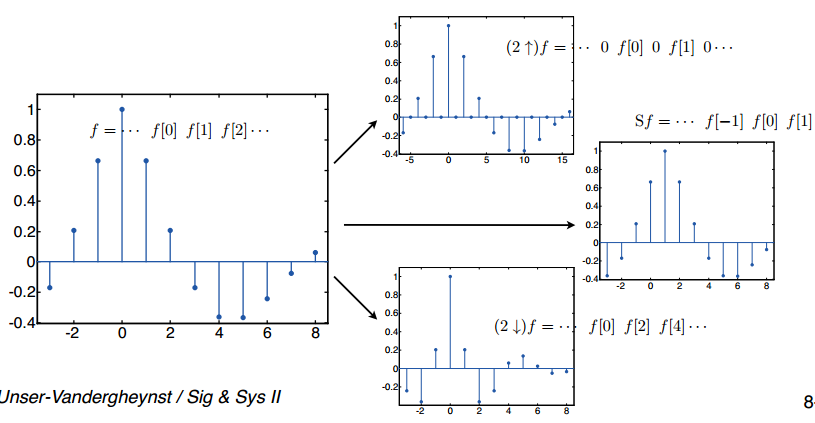
\includegraphics[width=\linewidth]{res/operateurs-echant.png}
\end{Figure}

% ============================= 

\section{Espaces vectoriels de signaux}

\begin{myitemize}
    \item Pas de notion de presure partout
    \item Pas de valeurs infinies
    \item Pas de continuité, dérivabilité, etc...
\end{myitemize}

\subsection*{Espace signaux à énergie finie}

$\el{2} = \left\{ f : \mathbb{Z}\rightarrow\mathbb{C} : \norm{f}_{l_2}^2 = \sum_{n\in\mathbb{Z}}|f[n]|^2 < \infty \right\}$

C'est un \textbf{espace de Hilbert} équipé du produit scalaire discret $\langle f, g \rangle_{\ell_2} = \sum_{n\in\mathbb{Z}} f[n]g^*[n]$

Exemple : exp. causale décroissante, $|a|<1, a^nu[n] \in \el{2}$

\textbf{Inégalité Cauchy-Schwarz} : \\
$\langle f, g \rangle_{\ell_2} \leq \norm{f}_{\ell_2} \norm{g}_{\ell_2} \: \forall f,g\in \el{2}$

\subsection*{Normes discrètes}

Normes-$\ell_p$, $p\in [1,\infty]$,

\begin{equation*}
    \norm{f}_{\ell_p} = 
    \begin{cases}
    \left( \sum_{n\in\mathbb{Z}} |f[n]|^p \right)^{\sfrac{1}{p}} & p \in [1,\infty[\\
    \sup_{n\in\mathbb{Z}}|f[n]| & p = \infty
\end{cases}\end{equation*}

\textbf{Propriétés norme}:
\begin{myitemize}
    \item Non-négativité : $\norm{f}_{\ell_p} \geq 0$
    \item Homogenéité : $\norm{\alpha\cdot f}_{\ell_p} = |\alpha| \norm{f}_{\ell_p} \: \forall \alpha\in\mathbb{C}$
    \item Inégalité triangulaire : $\norm{f+g}_{\ell_p} \leq \norm{f}_{\ell_p} + \norm{g}_{\ell_p}$
\end{myitemize}

\textbf{Hiérarchisation} : $\normel{f}{\infty} \leq \normel{f}{q} \leq \normel{f}{p} \leq  \normel{f}{1}$, pour tout signal $f$ et $1\leq p \leq q \leq \infty$

\subsection*{Espaces vectoriels discrets}

Espace $\el{p}, p\geq 1$ : 
\begin{equation*}
    \el{p} = \left\{ f: \mathbb{Z} \rightarrow \mathbb{R} : \normel{f}{p} < \infty \right\}
\end{equation*}

Ce sont des espaces de Banach. Cas particuliers :

\begin{myitemize}
    \item $\el{2}$ signaux discrets à énergie finie
    \item $\el{1}$ signaux discrets sommables (val abs)
    \item $\el{\infty}$ signaux discrets bornés
\end{myitemize}

\textbf{Imbrication} : $\el{1} \subseteq \el{p} \subseteq \el{q} \subseteq \el{\infty}$, pour $1\leq p \leq q \leq \infty$

\subsection*{Produit scalaire étendu}

\textbf{Déf} : $p,p' \in [1,\infty]$ forment une paire conjuguée si $\sfrac{1}{p} + \sfrac{1}{p'} = 1$

\begin{myitemize}
    \item Produit de dualité : pour $p,p'$ des indices conjugués et $f\in\el{p}, g\in\el{p'}$, $\langle ,g \rangle$ est une forme bilinéaire et continue
    
    \item Inégalité Hölder : pour tout $f\in\el{p}, g\in\el{p'}$, $p,p'$ des conjugués, on a $|\langle f,g \rangle| \leq \normel{f}{p}\normel{g}{p'}$
\end{myitemize}

\subsection*{Signaux bornés vs non-restreints}

Déf : le signal $f$ est dit : 
\begin{myitemize}
    \item borné : $\el{\infty}$
    \item à support fini $\mathcal{C}(\mathbb{Z})$ : $\exists n_0 \leq n_1 \in \mathbb{Z}$ t.q. $f_{[n_0\dots n_1]} = f \in \el{\infty}$
    \item localement sommable/borné : $f_{[-N\dots N]} \in \el{1} \subseteq \el{\infty} \: \forall N\in\mathbb{N}$, alors $f \in\mathcal{C'}(\mathbb{Z})=\mathbb{R}^\mathbb{Z}$
\end{myitemize}

\textbf{Propriété inclusion} $1\leq p\leq q \leq \infty$ : 
\begin{equation*}
    \mathcal{C}(\mathbb{Z}) \subseteq \dots \el{1} \subseteq \el{p} \subseteq \el{q} \subseteq \el{\infty} \subseteq \dots \subseteq \mathcal{C'}(\mathbb{Z})
\end{equation*}

% ============================= 

\section{Systèmes linéaires discrets}

\subsection*{Définition}

Les systèmes linéaires discrets sont des opérateurs linéaires qui agissent sur les signaux discrets: $f[n] \rightarrow$ \mybox{$T\{\cdot\}$} $\rightarrow g[n]$

Représentation : Système linéaire discret $T$ entièrement décrit par fonction de deux variables entières $H[n,k]$ t.q. $T\{f\} = \sum H[n,k] f[k]$

\subsection*{Systèmes LID}

Systèmes linéaires \textbf{invariants par décalage} : $T\{S^kf\} = S^kT\{f\}$

Un système est LID si et seulement si:
\begin{enum}
\item Il est linéaire
\item $H[n,k] = T\{\delta[\cdot-m] \}[n] = T\{\delta \}[n-m] = H[n-m,0]=h[n-m]$
\end{enum}

Autrement dit :

\begin{equation*}
    T \text{ est LID } \iff \exists h \text{ t.q. } T\{f \} = \sum_k h[n-m]f[m]
\end{equation*}

avec $h$ la \textbf{réponse impulsionnelle discrète}

Exemples: $S$ est LID avec $h=\delta[\cdot-1]$

\subsection*{Convolution discrète}

\begin{align*}
    (f*g)[n] & = \ssum_k f[k] \cdot g[n-k] = \langle f, g[n-\cdot ] \rangle \\
    & = \ssum_m f[n-m] \cdot g[m]
\end{align*}

Propriétés: commutativité, associativité, distributivité p.r. à addition. Impulsion discrète est éléments neutre : $(\delta * g)[n] = g[n]$.

Convolution pas forcément bien déf pour tout $f,g\in\mathcal{C'}(\mathbb{Z})$

\textbf{Relation convolution <-> rép. impuls. des sys LID}

\begin{align*}
    T\{f\}[n] & = T\{f*\delta\} = T\left\{\textstyle\sum_{k_0}f[k_0]\cdot\delta[n-k_0]\right\}\\
    & = \ssum_{k_0}f[k_0]\cdot h[n-k_0] = (f*h)[n]
\end{align*}

\subsection*{Systèmes RIF - RII}

Soit système LID spécifié par l'opérateur de convolution discret : $S_h : f \mapsto h*f$

Systèmes à réponse impulsionnelle finie : $\text{support}(h)$ est fini. 

Propriété : convo de signaux à support fini est à support fini, $h,f\in\mathcal{C}(\mathbb{Z}) \Rightarrow h*f \in\mathcal{C}(\mathbb{Z})$. En particulier, pour $h_1,h_2$ de longeur $N_1,N_2$, $h_1*h_2$ aura longeur max $(N_1+N_2-1)$

\textbf{Fonction transfer} : $S_h \text{ RIF } \iff \exists n_0 \text{ t.q. } H(z) = z^{-n_0}P(z^{-1}), P(X)$ un polynôme

\subsection*{Systèmes causaux}

Un \textbf{signal causal} (discret) $f$ est t.q. $f[n]=0 \: \forall n<0$

Un \textbf{système LID causal} $S_{h_+}$ est t.q. $h_+$ est causal

\textbf{Propriétés} :
\begin{myitemize}
    \item Convolution de signaux causaux est tjs causale
    \item Convolution de signaux causaux est tjs bien définie
\end{myitemize}

\subsection*{Stabilité des opérateurs LID}

\textbf{Définition} : L'opérateur de convolution $S_h, h \in\mathcal{C'}(\mathbb{Z})$ est $\ell_p\text{-stable}$ s'il existe une constante $0<C<\infty$ t.q. $\forall f\in\el{p}$ : 

\begin{equation*}
    \normel{S_h\{f\}}{p} = \normel{h*f}{p} \leq C\normel{f}{p}
\end{equation*}

\textbf{Conséquence} : 
\begin{equation*}
    S_h \text{ est } \ell_p\text{-stable}, f\in\el{p} \Rightarrow S_h\{f\} = h*f \in \el{p}
\end{equation*}

\textbf{Stabilité BIBO} : stabilité au sens de $\ell_\infty$

\textbf{Théorème BIBO stabilité} : $S_h$ est BIBO stable $\iff h \in\el{1}$ 

\textbf{Stabilité de composition} : au sens de $\ell_1$

\textbf{Théorème stabilité composition} : $S_h$ est $\ell_1\text{-stable} \iff h\in\el{1}$

\subsection*{Composition de systèmes LID}

\begin{myitemize}
    \item Mise en série (associativité) : $h = h_1 * \dots * h_n$
    \item Mise en parallèle (distribuvitivé) : $h = \sum_{k=1}^K a_kh_k$
\end{myitemize}

\subsection*{Algèbre des opérateurs LID}

Flemme.

\subsection*{Opérateur inverse}

\textbf{Définition Injectivité} : $S_h : \el{\infty}\rightarrow\el{\infty}$ est injectif si $S_h\{f_1\} = S_h\{f_2\}$ implique que $f_1=f_2$.

\textbf{Propriété} : $S_h$ est injectif sur $\el{\infty} \iff \exists g\in \el{1}$ tel que $h*g=\delta$, il admet alors un inverse de convolution $S_g=S_h^{-1}$  

\subsection*{Opérateur de convolution}

\textbf{Théorème} : $\forall f\in\el{p}, p\geq 1, h\in\el{1}$, on a $\normel{h*f}{p} \leq \normel{h}{1}\normel{f}{p}$

\textbf{Conséquence} : L'opérateur de convolution $S_h$ est $\ell_p\text{-stable}$

% ============================= 

\section*{Transformée en Z}

\textbf{Définition} : Soit $f$ signal discret, sa transformée en $z$ est déf par $F(z) = \sum_n f[n]z^{-n}$

\subsection*{Rayon de convergence}

$f$ est à \textbf{support semi-fini} ssi $\exists n_0$ tel que:

\begin{myitemize}
    \item $f[n] = 0 \: \forall n < n_0$ (support semi-fini positif). $F(z)$ est alors une série entière en $z^{-1}$ avec domaine de convergence : $\{z\in\mathbb{C} : |z| > \rho_+\}, \rho_+ = \limsup_{n\rightarrow\infty}|f[n]|^{1/n}$
    \item $f[n]=0 \:\forall n>n_0$ (support semi-fini négatif). $F(z)$ est alors une série entière en $z$ avec domaine de convergence : $\{z\in\mathbb{C} : |z| < \rho_-\}, \rho_- = 1/\limsup_{n\rightarrow\infty}|f[-n]|^{1/n}$
\end{myitemize}

\subsection*{Lien avec série Taylor}

\begin{myitemize}
\item Pour $f$ à support semi-positif et $\rho_+<\infty \Rightarrow z^{-n_0}F(z^{-1})$ est analytique dans disque $|z|<\rho_+$, $f[n]$ est donné par développ. Taylor autour de $z=0$: 
$f[n+n_0] = \frac{1}{n!}\frac{d^n}{dz^n}\left(z^{-n_0}F(z^{-1})\right)\rvert_{z=0}$

\item Pour $f$ à support semi-négatif et $\rho_- \neq 0 \Rightarrow z^{n_0}F(z)$ est analytique dans disque $|z|<\rho_-$ et on a le dévelop. Taylor en 0 : 
$f[n-n_0] = \frac{1}{n!}\frac{d^n}{dz^n}\left(z^{n_0}F(z)\right)\rvert_{z=0}$

\item Rappel: fonction analytique dans $D\subseteq \mathbb{C}$ si sa série de Taylor converge uniformément dans tout $D$
\end{myitemize}


% ============================= 

\section{Fonction de transfert}

\textbf{Pôles, zéros} : attention, $H(z)=z^{-d}$ ne possède pas de zéros ($z_0 \neq 0 \neq z_p)$.

\textbf{Causalité} : $S_h$ causal $\Rightarrow H(z)$ série entière en $z^{-1}$ (réciproque vraie mais avec il existe un sys causal). Il suffit de vérif que $\exists \rho $ t.q. $H(z)$ est analytique dans $|z|>\rho$

\textbf{Stabilité} : causalité + $\rho < 1 \Rightarrow$ stabilité. (si on admet $h$ anti-causal), LID réalisable stable $\iff$ poles pas sur cercle unité ; (alternativement, $h\in\el{1}$)

\textbf{Filtre réels} : $h=h^* \iff H(z)^* = H(z*)$, les zéros et pôles non réels doivent être pairs et symétrique par rapport à axe réel.

\textbf{Sys LID réalisable} : si $H(z) = z^{-n_0}P(z^{-1})/Q(z^{-1})$ avec $P,Q$ des polynomes premier entre eux. Autrement dit, si sys LID est décrit par équ. aux différences. 

\textbf{RIF/RII} : dès que $Q(z^{-1})$ n'est pas $z^{-d}$, $h$ nécessairement RII

\textbf{Stable + causal} : $H(z)$ doit avoir poles \textbf{à l'intérieur du cercle unité}.

\textbf{Phase linéaire} : poles et zéros symétriques par rapport au cercle unité, voir section \ref{phase_lineaire}

\textbf{Passe-tout} : de forme $H(z) = \gamma z^N P(z) / P^*(z^{-1})$, à tout zéro $z_{0,m}$ correspond un pole $z_{p,m} = 1/z^*_{0,m}$ et vice-versa.

% ==== : ===+ causal====================== 

\section{Equations aux différences}

$f[n]\rightarrow$ \mybox{LID} $\rightarrow g[n]$

\begin{align*}
    a_Ng[n-N] + \dots + a_0g[n] & = b_Mf[n-M] + \dots + b_0f[n]\\
    (a*g)[n] & = (b*f)[n]
\end{align*}

$S_a\{g\} = S_b\{f\} \rightarrow g = S_a^{-1}\{S_b\{f\}\} = a_{inv}*b*f=h*f\\
\Rightarrow \mathbf{h = a_{inv} * b}$

\subsection*{Inversion - Méthode temporelle}

Facorisation $S_a^{-1} = \frac{1}{a_0}(I-r_NS)^{-1}\dots(I-r_1)^{-1}$

$a_{inv} = \frac{1}{a_0} (h_N*\dots*h_1)$, réponse particulière $h=a_{inv}*b$

$h_k[n] = (I-r_kS)^{-1}[n]=(r_k)^nu[n] \quad\text{ si } |r_n|<1$

Condition BIBO-stable : $|r_k| \neq 1 \quad \forall k$

\subsection*{Inversion - Méthode domaine en Z}

On obtient une fraction rationelle :

$A(z)G(z)=B(z)F(z) \rightarrow H(z) = \frac{B(z)}{A(z)} = \frac{b_0 \prod_{m=1}^M(z-z_{0,m})}{a_0 \prod_{n=1}^N (z-z_{p,n})}$ 

Après factorisation, \textbf{décomposition en éléments simples} puis inversion des fonctions simples avec formulaire

\subsection*{Solution homogène - Conditions initiales}


$g_0[n] = C_1(r_1)^n + \dots + C_N(r_N)^n$, $C_i$ des const $\in\mathbb{R}$, $r_i$ les racines de $A(z)$

Racines multiples: $C_i \rightarrow Q_i[n]$, $i = 1,\dots,d$ pour d racines distinctes, de multiplicité $m_i$. $Q_i$ polynomes de degré $m_i-1$.

\subsection*{Circuits - Symboles graphiques}

\begin{Figure}
    \centering
    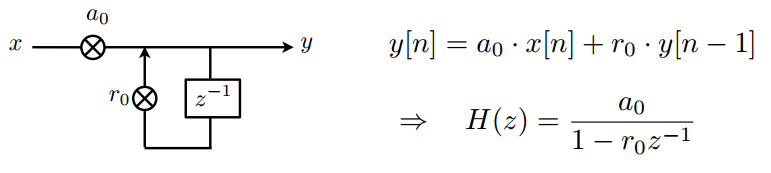
\includegraphics[width=\linewidth]{res/implementation-symboles.png}
\end{Figure}

% ============================= 

\section*{Fourier Discret}

\begin{Figure}
    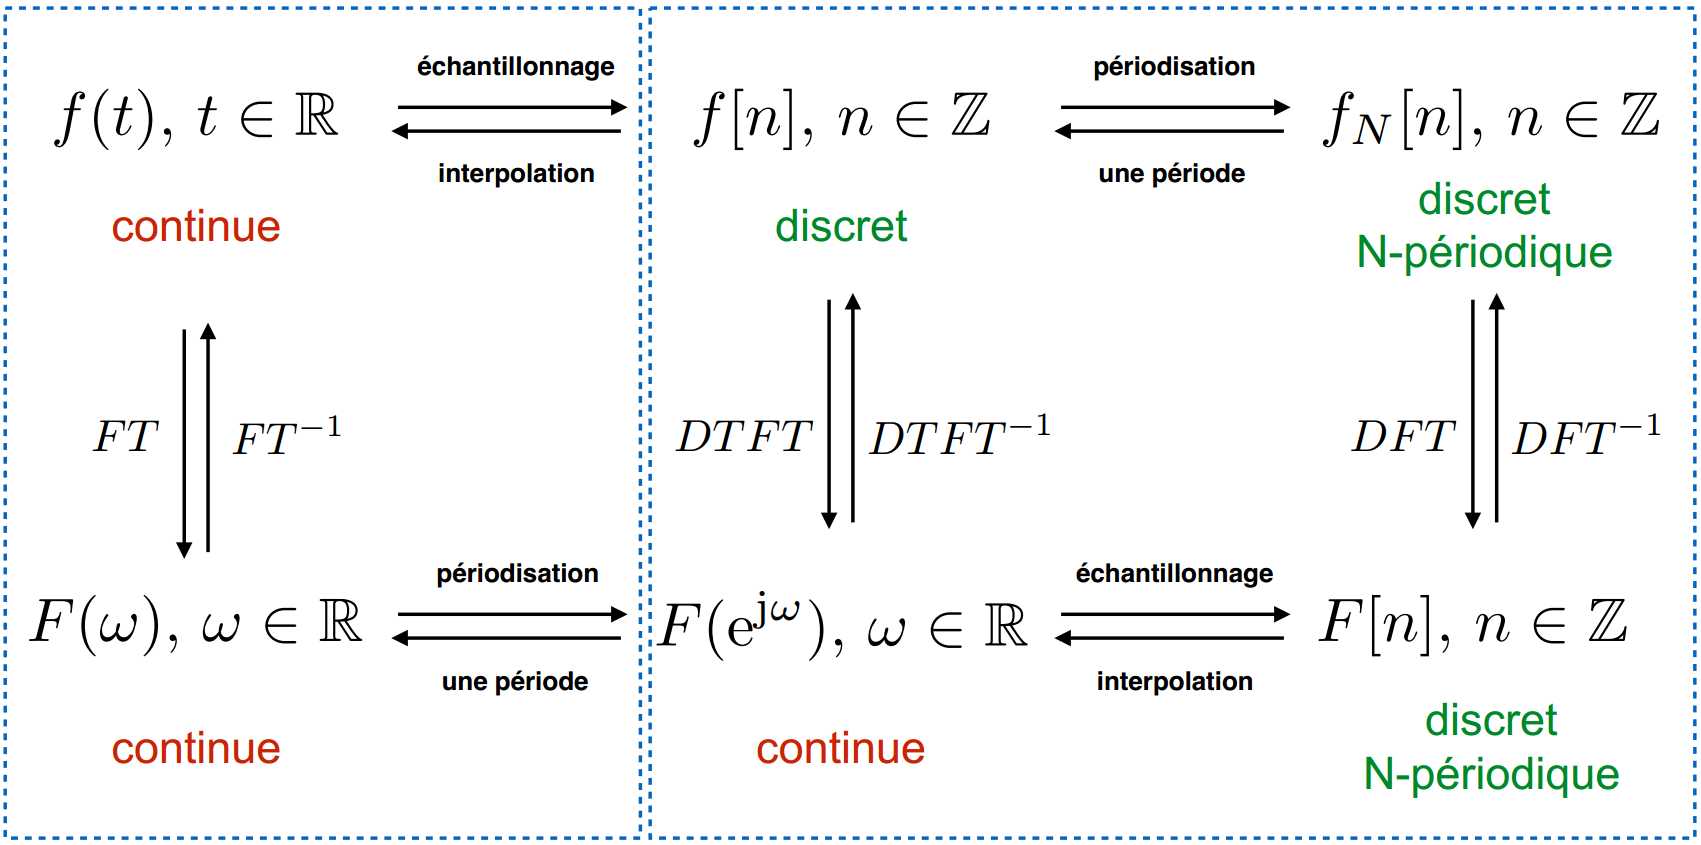
\includegraphics[width=\linewidth]{res/lien-transformees-fourier.png}
\end{Figure}

\textbf{DTFT} : transfo Fourier temps discret (déf et lien avec continu) : \\$\mathcal{F}_d\{f\}(\omega) = \mathcal{F}\{\sum_nf[n]\delta(\cdot-n)\}(\omega) = \sum_n f[n]e^{-j\omega n}$

\begin{myitemize}
    \item DTFT est signal $2\pi$-\textbf{périodique}
    \item Convergence assurée seulement si $f\in\el{1}$
\end{myitemize}

\textbf{Lien transfo en Z} : Pour $F(z)$ convergence sur cercle unité, on a : $F(e^ {j\omega}) = \mathcal{F}_d\{f\}(\omega)$

\textbf{Lien transfo continue} : on représente $f[n]$ en continu : $f_T(t) = \sum_n f[n] \cdot\delta(t-nT)$, on a $\mathcal{F}\{f_T\}(\omega) = F(e^{j\omega T})$. Si $f$ bande limitée, $\mathcal{F}\{f\}(\omega) = ???$

\textbf{Réponse fréquentielle système LID} : $S_h$, $H(e^{j\omega})=\mathcal{F}_d(\omega)$

\textbf{Stabilité} : $S_h$ est $\ell_2$-stable $\Leftrightarrow H_{max}<\infty$

\textbf{Invertibilité} : $S_h$ est inversible sur $\el{2} \Leftrightarrow H_{min} > 0$ et $S_h^{-1}: f\mapsto h_{inv}*f$, $h_{inv}[n] = \mathcal{F}_d^{-1}\left\{\frac{1}{H(e^{j\omega})}\right\}[n]$ 

\begin{Figure}
    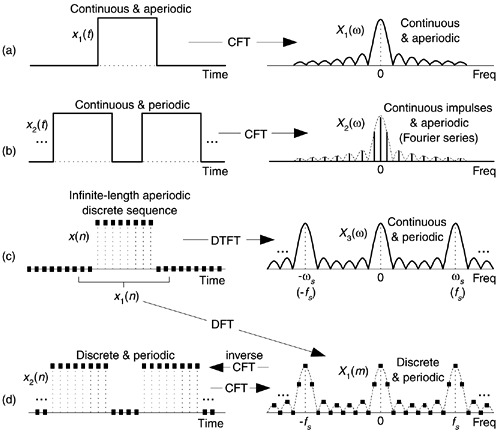
\includegraphics[width=\linewidth]{res/lien-transformees-exemple.jpg}
\end{Figure}

% ============================= 

\section{Transformée Fourier Discrète (DFT)}

$DFT\{f\}[m] = F[m] = \sum_{n=0}^{N-1}f[n]e^{-jm\frac{2\pi}{N}n}$

\textbf{Moyenne} : $m = F[0]/N$

\textbf{Lien continu} : $\sum_nf_N[n]\delta(t-nT) \fourierarrow \frac{2\pi}{NT}\sum_n F[n] \delta(\omega-n \frac{2\pi}{NT})$

\textbf{Lien DTFT} : $f[n]$ support fini, $f_N[n]$ sa version $N$-périodisée, on a $F(e^{j\omega_m}) = F_N[m]$ aux fréquences $\omega_m = m\frac{2\pi}{N}$, attention aliasing, sauf si $f[n]$ à support fini dans $[0\dots N-1]$

\textbf{Filtres} : réponse amplitude = $|H(e^{j\omega})|$, réponse en phase = $\operatorname{Arg}{H(e^{j\omega})}$

% ============================= 

\section{Fast Fourier  Transform (FFT)}

$8N^2$ opérations pour calculer DFT.

Idée : si facto $N=pq$, alors $F[m] = \sum_{n=1}^{N-1} f[n] \cdot W_N^{mn}, W_N^{mn} = e^{-j\frac{2\pi}{N}}$

\textbf{Algorithme diatique} : pour $N=2M$, 
\begin{align*}
    F[m] &= F_0[m] + W_N^m F_1[m]\\
    F_0[m] &= \ssum_{n=0}^{N/2-1} f[2n]\cdot W_{N/2}^{mn}  \\
    F_1[m] &= \ssum_{n=0}^{N/2-1}f[2n+1] \cdot W_{N/2}^{mn}
\end{align*}

puis on divise les fréq en 2 ensembles $0,1,\dots,(N/2-1)$ et $(N/2),\dots,(N-1)$, puis : $\begin{cases}F[m] = F_0[m] + W_N^m\cdot F_1[m]\\F[m+N/2]=F_0[m]-W_N^m\cdot F_1[m]\end{cases}, \: m=0,1,\dots,(N/2-1)$

% ============================= 

\section{Analyse fréquentielle }

\subsection*{Implémentation filtrage}

\textbf{Filtrage rapide} : ne pas calculer convo $h*f$, mais DFT de $h$ et $f$ (avec zero padding), les multiplier, puis DFT$^{-1}$. 

\subsection*{Analyse filtres numériques}

\textbf{Réponse fréquentielle sys LID} : $H(e^{j\omega}) = A_H(\omega) \cdot e^{j\Phi_h(\omega)}$

\textbf{Types de filtres} : passe-bas, -haut, -bande, -tout, toujours entre $-\pi,\pi$

\textbf{Distorsions} : 
\begin{myitemize}
    \item $\omega_c$ est la fréquence au centre de bande passante
    \item D'amplitude :$\operatorname{Att}_H(\omega) = 20log_10(A_H(\omega)/A_H(\omega_c))$
    \item De phase : distorsion est $\operatorname{TPG}_h(\omega)-\operatorname{TPG}_h(\omega_c)$, \textbf{Temps de propagation de groupe} :
    \begin{equation*}
        \operatorname{TPG}_h(\omega) = -\frac{d}{d\omega} \Phi_H(\omega) = - \operatorname{Re}\left( e^{j\omega} \frac{H'(e^{j\omega}}{H(e^{j\omega})} \right)
    \end{equation*}
    \item Additivité par convolution pour atténuation et TGP
\end{myitemize}

\subsection*{Filtres à phase linéaire} \label{phase_lineaire}

\textbf{Phase linéaire} : pas de distorsion de phase, $\operatorname{TPG}_h(\omega) = K \Leftrightarrow \Phi_H(\omega) = \theta_0 - K\omega$

\textbf{Filtres réalisables phase linéaire} : 
\begin{equation*}
    H(z) = \epsilon z^{-N} H(z^{-1}), \epsilon \in \{-1,1\} \Leftrightarrow \operatorname{TPG}_h(\omega) = N/2
\end{equation*}

on a $\epsilon = 1$ pour les filtres symétriques, $-1$ pour anti-symétrique (axe pas forcément en 0, entre 2 points possible)

\subsection*{Synthèse à partir d'un filtre analogique}

Bonnes propriétés des filtres continus $\rightarrow$ les convertir en discret. Pour $\hat h = \mathcal{F}\{h(t)\}$ la transfo en continu, on veut un filtre discret tel que $H(e^{j\omega}) \approx \hat h(\omega)$ sur de larges bandes.

\textbf{Transformaiton bilinéaire} : on approx avec fonction $(2\pi/T)$-péioridique $H_{bilineaire}(e^{j\omega}) = \hat h\left(\frac{2}{jT}\frac{1-e^{-j\omega}}{1+e^{-e\omega}}\right)$. Propriétés : $\hat h$ est frac rationnelle en $j\omega$ et BIBO stable $\Leftrightarrow$ $H_{bilineaire}$ est frac. rationnelle en $e^{j\omega}$ et BIBO stable.

\subsection*{Synthèse directe de filtres numériques}

On représente la réponse fréquentielle avec cercle unité, zéros effet attractif, poles effet répulsif.

On peut synthétiser avec différents critères ($L_2$, erreur moyenne)...

% ============================= 

\section{Probabilités}

Notion d'aléatoire : i) réception de valeurs issues d'un processus possiblement déterministe mais inconnu ii) bruit des systèmes physiques

\textbf{Notations} : $X, \mathbf{X}, X(\cdot), X[\cdot]$ contreparties aléatoires de $x\in\mathbb{R}, \mathbf{x}\in\mathbb{R^Z}, x(\cdot) :\mathbb{R}\rightarrow\mathbb{R}, x[\cdot]:\mathbb{Z}\rightarrow\mathbb{R}$.

\textbf{Densité de probabilités} : $p_X:\mathbb{R}\rightarrow\mathbb{R_+}$ caractérise variables aléatoires, permet calculer probabilité de tout événement $E\subseteq\mathbb{R} : \text{Prob}(X\in E) = \int_E p_X(x)dx$

\begin{myitemize}
    \item $p_{uni}(x; a,b) = \frac{1}{a-b}\text{rect}(\frac{x-a}{b-a}-\sfrac{1}{2})$
    \item $X \sim \mathcal{N}(\mu,\sigma) \Leftrightarrow p_X(x) = \frac{1}{\sigma\sqrt{2\pi}}\exp({-\frac{(x-\mu)^2}{2\sigma^2}})$
    \item $p_{exp}(x;\lambda) = \lambda e^{-\lambda x} u(x)$
\end{myitemize}

\textbf{Espérance} : Soit $f:\mathbb{R}\rightarrow\mathbb{R}$ une transformation (fonction mesurable) de la VA $X$, la valeur moyenne de $f(X)$ est :
\begin{equation*}
    \mathbb{E}_X\left\{f(X)\right\} = \int_\mathbb{R} f(x)p_X(x)dx = \langle p_X, f \rangle
\end{equation*}

pour $X,Y$ indépendantes, $\expected{XY}=\expected{X}\expected{Y}$

\textbf{Moments} : On calcule $\mathbb{E}_X\left\{f(X)\right\}$ avec différents $f$ : $\mu_{X,0} \leftrightarrow f(X) = 1,\quad \mu_X = \mu_{X,1} \leftrightarrow f(X) = X,\quad \mu_{X,n}\leftrightarrow f(X) = X^n,\quad \sigma_X^2\leftrightarrow f(X)=(X-\mu_X)^2$

\textbf{Lien continu-discret} : pour $X$ VA ne prenant que des valeurs discrètes $(x_n)_{n=1}^N$, on exprime la densité de probas avec Diracs pondérés $p_X(x) = \sum_{n=1}^N P(X=x_n) \cdot \delta(x-x_n)$

\textbf{Vecteurs aléatoires} : $\textbf{X}=(X_1,\dots,X_N)$ où $X_i$ sont des VA scalaires, elles ont une densité de probas $p_\mathbf{X} : \mathbb{R^N}\rightarrow\mathbb{R}_+$, vecteur moyenne (par composante) $\mathbf{\mu_X} = \mathbb{E}\{\mathbf{X}\}$, matrice covariance $\mathbf{C_X} = \mathbb{E}\{(\mathbf{X}-\mathbf{\mu_X})((\mathbf{X}-\mathbf{\mu_X})^\intercal\}\in\mathbb{R}^{N\times N}, (\mathbf{C_X})_{m,n} = \mathbb{E}\{X_mX_n\}$

\quad $\rightarrow$ Exemple loi multivariée Gaussienne $p_\mathbf{X}(\mathbf{x}) = \exp(-(\mathbf{x-\mu})^\intercal \mathbf{C}^{-1} (\mathbf{x}-\mathbf{\mu})/2)/\sqrt{2\pi \det(\mathbf{C})}$

\textbf{Indépendance} : vecteur aléatoire $\mathbf{X}=(X,Y)$, $X$ et $Y$ sont des lois indépendantes $\Leftrightarrow p_\mathbf{X}(x,y) = p_X(x)p_Y(y)$

\textbf{Probas conditionnelles} : pour $\mathbf{X} = (X,Y)$, Bayes donne $p_\mathbf{X}(x,y) = p_{X,Y}(x,y) = p_{X|Y}(x|y) p_Y(y) = p_{Y|X}(x|y) p_X(x)$, avec la loi réduite $p_X(x)=\int_\mathbb{R}p_{X,Y}(x,y)dy$

\subsection*{Fonction caractéristique}
\begin{equation*}
    P_X(\omega) = \mathbb{E}\{e^{-j\omega X}\} = \int_\mathbb{R} p_X(x) e^{-j\omega x} dx = \mathcal{F}\{p_X\}(\omega)
\end{equation*}

\textbf{Théorème} : soient $X_1,\dots,X_N$ des variables \textbf{indépendantes} de lois $p_1(x), \dots, p_N(x)$ et soit $Y=X_1+\dots+X_N$, alors on a $p_Y(y) = (p_1 * \dots * p_N)(y)$, car $P_Y(\omega) = \prod_{i=1}^N P_{X_i}(\omega)$

\textbf{Cas discret} : pour $X$ VA discrète, on exprime sa pdf avec train Dirac : $p_X(x) = \sum_n \text{Prob}(X=n)\delta(x-n)$, on a donc sa fonc. caractéristique : \[P_X(\omega) = \ssum_n \text{Prob}(X=n) e^{-j\omega n} = \mathcal{F}_d\{\text{Prob}(X=n)\}(\omega)\]

% ============================= 

\section{Processus aléatoires}

\textbf{Signaux aléatoires} : à temps discret $X[\cdot]$ est un vect de dim infinie de vecteurs de VA $(\dots, X[n-1], X[n], X[n+1], \dots)$. A temps continu $X(\cdot)$ est la limite du signal discret pour des échant. avec $T\rightarrow 0$ 

\textbf{Idée} : même si signal déterministe, ne pas connaître comment il est généré = modéliser comme réalisation d'un tirage aléatoire

\textbf{Stationnarité sens strict} : n'importe quelle espérance est indép. du point de réf temporel

\textbf{Stationnarité sens large (SSL)} : indépendance du point de réf. temporel pour stats d'ordre 1 et 2 (moyenne et autocorrélation) : 
\[ \begin{cases}
\expected{X(t)} = \text{cst}\:\forall t\in\mathbb{R} \\
\expected{X(t)X(\tau)^*} = \rho_X(t-\tau)\:\forall t,\tau\in\mathbb{R}
\end{cases}\]

\textbf{Ergodicité} : toutes les moyennes statistiques de $X$ peuvent être déduites à partir d'une réalisation quelconque $x(\cdot)$, automatiquement stationnaire au sens strict

\textbf{Temps continu/discret} : échantillonnage $X[n]=X(nT)$ d'un signal statio $X(\cdot)$ donne un signal discret statio. L'interpolation $X_{int}(t = \sum_n X[n] \varphi(t/T-n)$ de $X[\cdot]$ statio n'est statio que si $\varphi(t) = \sinc(t)$.

\subsection*{Densité spectrale de puissance (DSP)}
A priori, $x(\cdot) \notin L_1(\mathbb{R})$, donc on borne le support $X_A(t) = \text{rect}(t/A)\cdot X(t)$ pour donner sens à $\hat X_A=\mathcal{F}\{X_A\}$. La densité spectrale de puissance $S_x$ du processus $X(t)$ est : $S_X(\omega) = \lim_{A\rightarrow\infty} \frac{1}{A}\expected{|\hat X_A(\omega)|^2}$. $\int_{\omega_1}^{\omega_2} S_X(\omega) \frac{d\omega}{2\pi}$ est contrib des fréq $[\omega_1,\omega_2]$ à la puissance moyenne du signal.

\textbf{Wiener Khintchine} : voir formulaire

\textbf{DSP signal filtré} : signal SSL $X(t)$, signal filtré $Y=h*X$ est aussi SSL et on a : 
\begin{equation*}
    S_Y(\omega) = |H(\omega)|^2 S_X(\omega)
\end{equation*}

avec $|H(\omega)|^2 = \mathcal{F}\{h*h^\vee\}$ la transfo de autocorrélation de $h$.

\subsection*{Bruit blanc}

\textbf{Bruit blanc continu} : $B(t)$ idéalisation mathématique d'un signal stationnaire à moyenne nulle avec DSP constante (indépendance échantillons) : $S_B(\omega) = \sigma_0^2 \Leftrightarrow \rho_B(t) = \sigma_0^2 \cdot \delta(t)$

\textbf{Bruit blanc discret} : $B[n]$ signal moyenne nulle, statio, indépendance échant, $\rho_B[n]=\sigma_0^2\delta[n]$

\textbf{Mouvement Brownien} (standard) : intégrale de $B(t)$, processus Gaussien t.q. $\expected{|X(t)-X(t')|^2}=C|t-t'|$, non statio mais ses acroissements le sont.

% ============================= 

\section{Information}

\textbf{Idée} : quantifier information relié à probabilité d'occurence, un msg de grande proba véhicule peu d'info 

\textbf{Information} $I(p) = -\log_a(p), a>1$ = fonction décroissante de $p$. Deux msg de probas $p,q \rightarrow I(p\cdot q) = I(p)+I(q)$  

\textbf{Interprétation} : computationel, info d'un message numérique est le nombre minimal $b$ de bits pour le stocker. Ex: msg de $n$ valeurs équiprobables est $b=\geq{\log_2n}$ bits. 

\textbf{Entropie source} : Source de msg décrite par VA discrète $X$ t.q. $P(X=x_k)=p_k$, l'entropie de la source est \textbf{l'information moyenne} par message : $H_X = -\sum_k p_k \log_2p_k$. Cas continu : \textbf{entropie différentielle} : $H_X = \expected{-\log_2p_X(x)}$

\textbf{Répartitions à entropie maximale} : sous contraintes: 
\begin{myitemize}
    \item Nb fini de valeurs possibles : distrib uniforme
    \item Energie moyenne finie $\expected{\norm{X}^2} < \infty$ : Gaussien discret
    \item Positivité et moyenne finie : exponentielle discrète
\end{myitemize}

\textbf{Information commune} : corrélation généralisée, $X,Y$ 2 sources aléatoires, si indép alors $H_{X,Y}=H_X+H_Y$, l'information commune est $I_{X,Y} = H_X+H_Y-H_{X,Y}$

\textbf{Capacité canal communication} : info commune entre émetteur-récepteur, capacité max d'un canal de largeur de bande $B$ [Hz] perturbé par bruit additif : $C = B\log_2(1+\text{RSB})$ bits/s. RSB \textbf{rapport signal sur bruit} = puiss. moy. signal divisée par puiss. moy. bruit vu par récepteur. 


% ============================= 

\section{Filtrage signaux bruités}

\textbf{Estimation signaux} : bruit $b$ additif, décorrélé du signal, moyenne nulle, signal reçu par récepteur $y(t) = x(t) + b(t)$. Sévérité perturbation quantifiée par rapport signal à bruit :
\begin{equation*}
    \text{RSB}_{dB} = 10\log_{10}\left(\frac{\expected{|X(t)|^2}}{\expected{|B(t)|^2}}\right)
\end{equation*}

\textbf{Filtrage accordé} : pour input discret, $x(t)=\sum_nf[n]\varphi(t-nT)$; garantit RSB maximisé aux instants d'échantillonnage, filtre optimal $H(\omega) = \Phi(-\omega)/S_b(\omega)$

\textbf{Filtre Wiener-Hopf} : pour $S_X, S_B$ connus, version réelle (non idéale) qui minimise la puissance moyenne de l'erreur: $H_W(\omega) = S_X(\omega)/(S_X(\omega)+S_B(\omega))$

